\documentclass[a4paper,twoside,11pt]{article}
\usepackage{a4wide,graphicx,fancyhdr,amsmath,amssymb,placeins}
\usepackage{listings}
\usepackage{color}
\usepackage{enumitem}
\usepackage{amsmath}
\usepackage{textcomp}
\usepackage{caption,subcaption}
\usepackage{placeins}

%----------------------- Macros and Definitions --------------------------

\setlength\headheight{20pt}
\addtolength\topmargin{-10pt}
\addtolength\footskip{20pt}

\newcommand{\N}{\mathbb{N}}
\newcommand{\ch}{\mathcal{CH}}
\newcommand{\cpp}{{\tt C++} }

\newcommand{\solution}[1][todo]{\noindent{\bf Solution to Exercise #1:}}
\newcommand{\todo}[1]{{\Large\sc\textcolor{red}{#1}}}

\renewcommand{\lstlistingname}{Codeblock}
\captionsetup[lstlisting]{font={small,tt}}

\fancypagestyle{plain}{%
\fancyhf{}
\fancyhead[LO,RE]{\sffamily\bfseries\large technische universiteit eindhoven}
\fancyhead[RO,LE]{\sffamily\bfseries\large 2IW02 RTSD}
\fancyfoot[LO,RE]{\sffamily\bfseries\large department of mathematics and computer science}
\fancyfoot[RO,LE]{\sffamily\bfseries\thepage}
\renewcommand{\headrulewidth}{0pt}
\renewcommand{\footrulewidth}{0pt}
}

\pagestyle{fancy}
\fancyhf{}
\fancyhead[RO,LE]{\sffamily\bfseries\large technische universiteit eindhoven}
\fancyhead[LO,RE]{\sffamily\bfseries\large 2IW02 RTSD}
\fancyfoot[LO,RE]{\sffamily\bfseries\large department of mathematics and computer science}
\fancyfoot[RO,LE]{\sffamily\bfseries\thepage}
\renewcommand{\headrulewidth}{1pt}
\renewcommand{\footrulewidth}{0pt}

%-------------------------------- Title ----------------------------------

\title{\vspace{-\baselineskip}\sffamily\bfseries Exercise 2}
\author{
	Rick Veens \qquad Studentno: 0912292\\
	\texttt{r.veens@student.tue.nl}
	\and
	Huib Donkers \qquad Studentno: 0769015\\
	\texttt{h.t.donkers@student.tue.nl}
}

\date{\today}

\definecolor{listinggray}{gray}{0.9}
\definecolor{lbcolor}{rgb}{0.9,0.9,0.9}
\lstset{
backgroundcolor=\color{lbcolor},
    tabsize=4,    
%   rulecolor=,
    language=[GNU]C++,
        basicstyle=\scriptsize,
        upquote=true,
        aboveskip={1.5\baselineskip},
        columns=fixed,
        showstringspaces=false,
        extendedchars=false,
        breaklines=true,
        prebreak = \raisebox{0ex}[0ex][0ex]{\ensuremath{\hookleftarrow}},
        frame=single,
        numbers=left,
        showtabs=false,
        showspaces=false,
        showstringspaces=false,
        identifierstyle=\ttfamily,
        keywordstyle=\color[rgb]{0,0,1},
        commentstyle=\color[rgb]{0.026,0.112,0.095},
        stringstyle=\color[rgb]{0.627,0.126,0.941},
        numberstyle=\color[rgb]{0.205, 0.142, 0.73},
%        \lstdefinestyle{C++}{language=C++,style=numbers}’.
}

% geen stomme indents bij \par
\setlength{\parindent}{0cm}

%--------------------------------- Text ----------------------------------

\begin{document}
\maketitle

\section{Timers}
\subsection{Model}
The model is shown in figure~\ref{fig:timermodel}, and code used for the first two tests in codeblock~\ref{code:timer}. The improved code used for the third test is shown in codeblock~\ref{code:timer2}. We used \texttt{octave} to parse the output as csv and perform some statistical analysis.

\begin{lstlisting}[caption=Pcode::execute, label=code:timer, language=C++]
void Pcode::execute()
{
  // protected region execute code on begin
	static struct timespec t1;


	struct timespec t2;
	struct timespec res;

	clock_gettime(CLOCK_REALTIME, &t2);
	clock_getres(CLOCK_REALTIME, &res);
	//long int elapsedTime = (t2.tv_usec - t1.tv_usec);

	printf("%ld.%.9ld, %ld.%.9ld, %ld.%.9ld\n", res.tv_sec, res.tv_nsec, t2.tv_sec, t2.tv_nsec, t1.tv_sec, t1.tv_nsec);

	t1 = t2;

	// protected region execute code end
}
\end{lstlisting}
\begin{lstlisting}[caption=Pcode::execute (improved), label=code:timer2, language=C++]
todo
\end{lstlisting}

\begin{figure}
 \centering
 \begin{subfigure}{\textwidth}
  \centering
  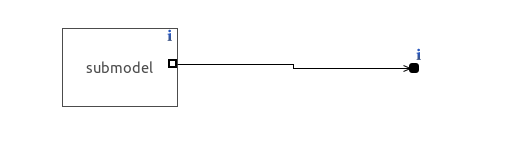
\includegraphics[width=0.8\textwidth]{./img/timer-mainmodel.png}
  \caption{Main model.}
 \end{subfigure}
 \begin{subfigure}{\textwidth}
  \centering
  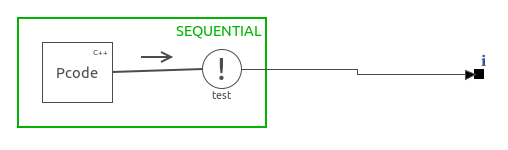
\includegraphics[width=0.8\textwidth]{./img/timer-submodel.png}
  \caption{submodel}
 \end{subfigure}
 \caption{Model used for testing the timer}
 \label{fig:timermodel}
\end{figure}

\FloatBarrier
\subsection{Questions} \label{sec:1_4}
\begin{enumerate}
 \item Measured over $1522$ intervals, the variation is $3.667 \cdot 10^{-8}$ s$^2$ or $0.03667$ ms$^2$. Since the clock resolution of QNX in virtual box ($0.000999848$ s) is so much larger than the observed variation, our measurements are not accurate enough to result in a variation that is representative for the actual variation. With a clock resolution of $0.000999848$ s, and a timer that ticks every $0.250000000$ s without jitter, we expect $\lceil 0.25/0.000999848 \rceil - 0.25/0.000999848 = 96.2\%$ of the measurements to be $\lfloor 0.25/0.000999848 \rfloor \cdot 0.000999848 = 0.249962$ s, and the other $3.8\%$ to be $\lceil 0.25/0.000999848 \rceil \cdot 0.000999848 = 0.250962$ s. In $1522$ measurements we found $96.2\%$ of the intervals to be $0.249962$ s and $3.8\%$ $0.250962$ s. Therefore, our measurements do not provide evidence of jitter.
 
 Up to a jitter bounded by $0.250000 - 0.249962 = 0.00038$ s $= 380$ $\mu$s, we would still expect the same results. For larger jitter, we would expect more and more measurements to be $0.248962$ s. So we can strengthen our claim: our measurements do not provide evidence of jitter larger than $380$ $\mu$s.
 
 We performed a second series of measurements, this time with the timer interval set to $0.249962$, an exact multiple of the clock resolution. We measured $1967$ intervals. With this configuration, we are likely to pick up on jitter with a variation larger than $(0.000999848/1967 \cdot 10^6)^2 \approx 0.258$ $\mu$s$^2$.
 
 Results of the second test is shown in figure~\ref{fig:interval-jitter}. This shows that there is indeed jitter. The variation of our measurements is $0.06$ ms$^2$.
 
 For a third test we used a method of timing with a resolution that is much higher: \texttt{ClockCycles()} from \texttt{sys/neutrino.h}. We can retrieve the number of clock cycles per second, so we can deduce how much time has passed if we know how many clock cycles passed. We measured $3339$ intervals using this method. The distribution of intervals is shown in figure~\ref{fig:interval-jitter2}. We can clearly see hoe the jitter behaves. It is still distributed somewhat discretely, but smaller deviations are now clearly shown. In this test the variation of the measurements is $7.814$ ms$^2$.
 
 \item This jitter is the result of simulating a real time OS in an environment that is not real time. Since the host OS decided when the virtual OS can run, and the host OS cannot guarantee to meet real time requirements, the virtual OS is unable to meet those requirements either.
 
 \item We observe from figure~\ref{fig:interval-jitter} that the timer tick is occasionally delayed by more than $1$ ms. Such a delay is not acceptable in many real time applications. \todo{Example.}
 
 \item No. Our virtual machines run on a non real time OS (GNU/Linux), so it can happen that the host OS is very busy with tasks that have a higher priority than the virtual machines, postponing execution of the real time OS unboundedly, disabling QNX to meet its real time requirements.
 
\end{enumerate}

\begin{figure}
 \centering
 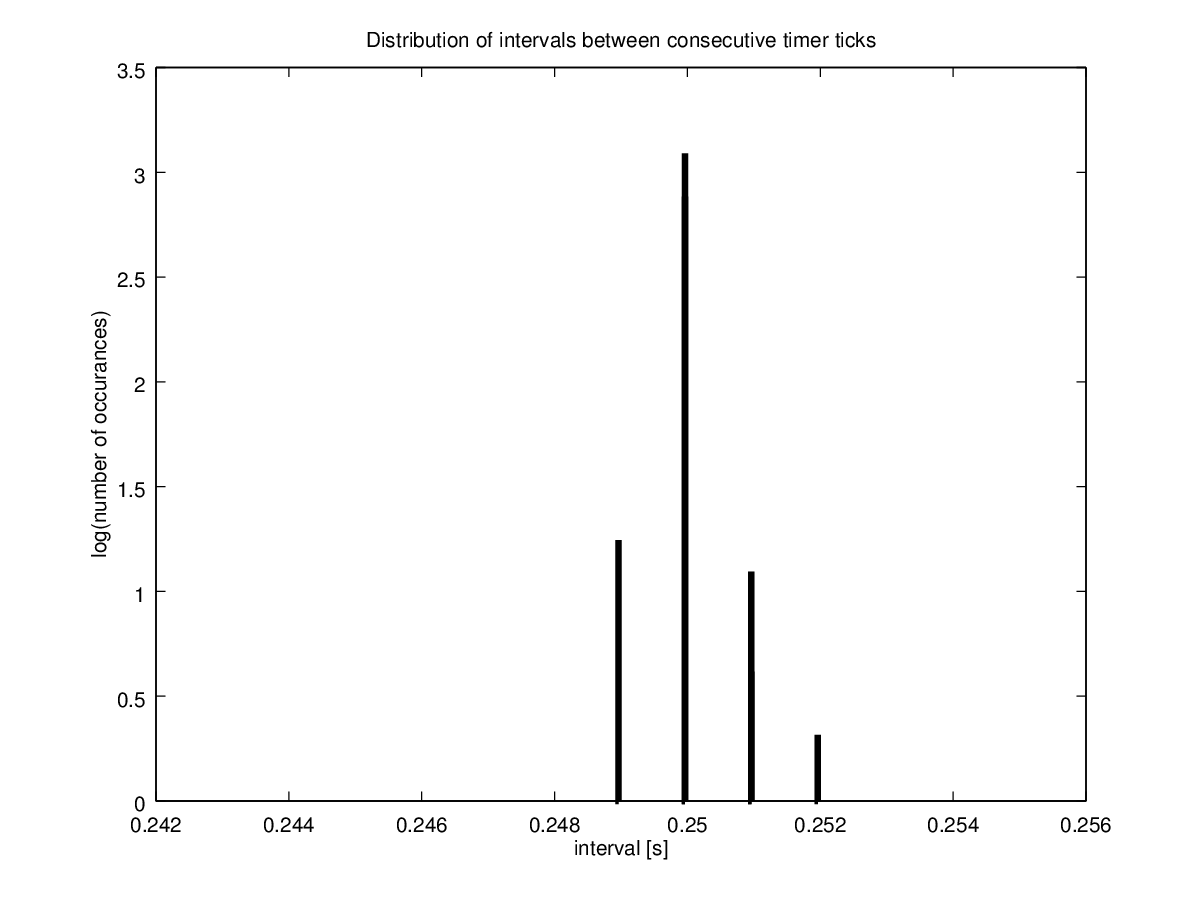
\includegraphics[width=0.8\textwidth]{./img/interval-jitter.png}
 \caption{Distribution of intervals in the second test.}
 \label{fig:interval-jitter}
\end{figure}
\begin{figure}
 \centering
 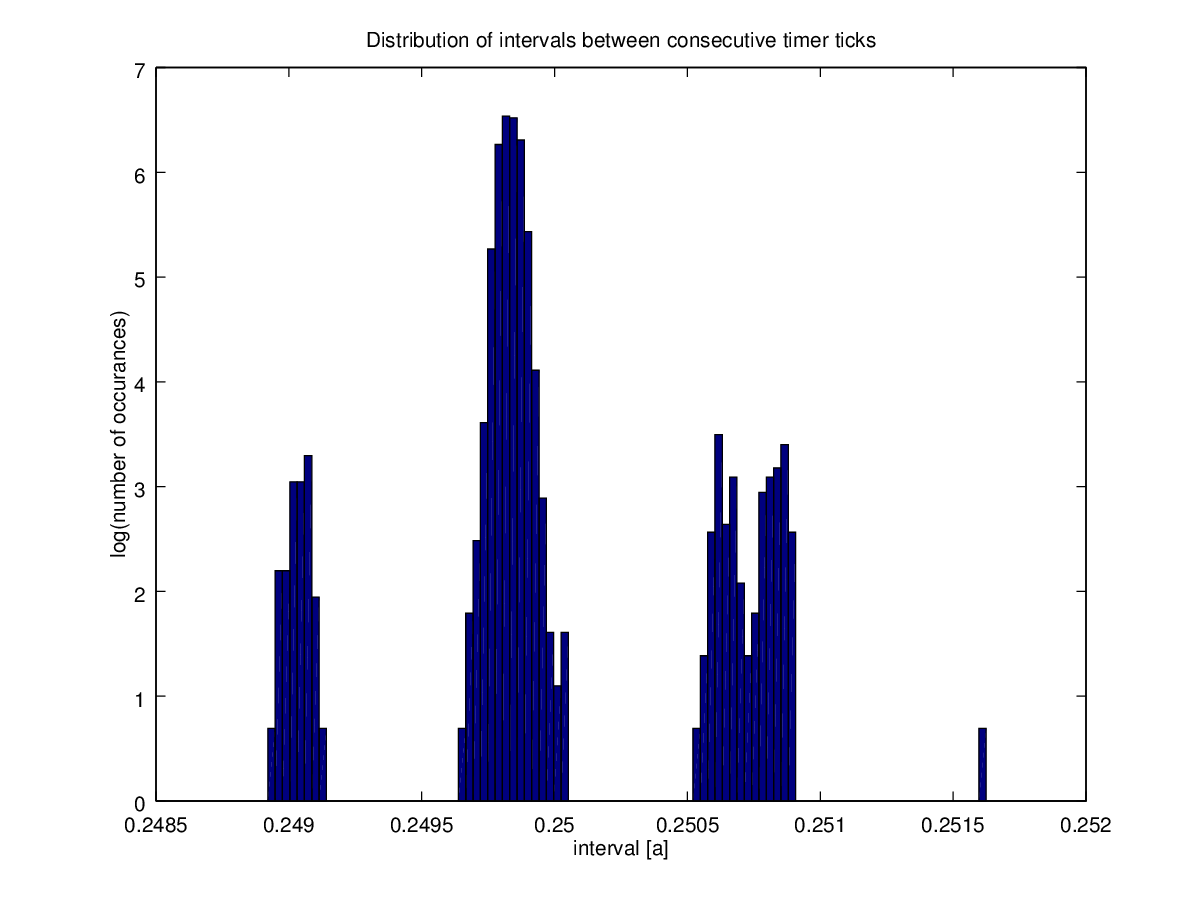
\includegraphics[width=0.8\textwidth]{./img/interval-jitter2.png}
 \caption{Distribution of intervals in the third test.}
 \label{fig:interval-jitter2}
\end{figure}

\FloatBarrier
\subsection{Validation}
We used the clock cycle approach, as described in section~\ref{sec:1_4} answer 1, to determine the exact interval.

\subsection{Questions}
\begin{enumerate}
 \item \todo{todo}
 \item \todo{todo}
 \item \todo{todo}
\end{enumerate}

\section{JIWYIO Linkdrivers}
\subsection{JIWYIO driver components}
\todo{Uitleg}

\subsection{Questions}
\begin{enumerate}
 \item \todo{todo}
 \item \todo{What!? ... You want us to tell you how the tool should work? This isn't software specification, and even worse, the tool is not the subject, it's the tool...}
 \item The most obvious drawback is of course that you need to do the exact same edits every time you generate code from the models. Another drawback is that you have to adapt your code to run simulations for testing. It is not possible to test the actual code that will be run in the real environment.
\end{enumerate}

\subsection{JIWYIO driver components in the lab}
\todo{Notes uitwerken}

run 1: 4Hz, timer_test1.csv - oscilloscope: 500.0 ms (sometimes 501.0 or 499.0)

run 2: 100Hz, timer_test2.csv - oscilloscope: 20.0 ms

\subsection{Questions}
\begin{enumerate}
 \item \todo{todo}
 \item \todo{todo}
\end{enumerate}

\section{Controlling JIWY with QNX \& CSP}
\subsection{Test at the lab}
\todo{report}

\subsection{Questions}
\begin{enumerate}
 \item \todo{todo}
 \item \todo{todo}
\end{enumerate}

\subsection{Further functionality}
\todo{explain we didn't have time and it's not our fault}

\subsection{Questions}
\begin{enumerate}
 \item \todo{todo}
 \item \todo{todo}
 \item \todo{todo}
 \item \todo{todo}
\end{enumerate}

\end{document}
